%!TEX TS-program =  pdflatex 


\documentclass{amsart}
\usepackage{array}
\newcolumntype{P}[1]{>{\raggedright\let\newline\\\arraybackslash\hspace{0pt}}m{#1}}
\usepackage{graphicx,verbatim, amsmath, amssymb, amsthm, amsfonts, epsfig, amsxtra,ifthen,mathtools,epstopdf,caption,enumerate,hyperref,hhline,bbm,capt-of,longtable}	
\DeclareFontFamily{U}{mathx}{\hyphenchar\font45}
\DeclareFontShape{U}{mathx}{m}{n}{<-> mathx10}{}
\DeclareSymbolFont{mathx}{U}{mathx}{m}{n}
\DeclareMathAccent{\widebar}{0}{mathx}{"73}
\epstopdfsetup{suffix=}
\DeclareGraphicsExtensions{.ps}
\DeclareGraphicsRule{.ps}{pdf}{.pdf}{`ps2pdf -dEPSCrop -dNOSAFER #1 \noexpand\OutputFile}

\newtheorem{proposition}{Proposition}[section]
\newtheorem{theorem}[proposition]{Theorem}
\newtheorem{corollary}[proposition]{Corollary}
\newtheorem{lemma}[proposition]{Lemma}
\newtheorem{prop}[proposition]{Proposition}
\newtheorem{cor}[proposition]{Corollary}
\newtheorem{thm}[proposition]{Theorem}
\newtheorem{conj}[proposition]{Conjecture}
\newtheorem{phen}{Phenomenon}

\renewcommand\thephen{\Roman{phen}}

\theoremstyle{definition}
\newtheorem{example}[proposition]{Example}
\newtheorem{definition}[proposition]{Definition}
\newtheorem{question}[proposition]{Question}

\theoremstyle{remark}
\newtheorem{remark}[proposition]{Remark}
\newtheorem{problem}[proposition]{Problem}

\numberwithin{equation}{section}
\usepackage[usenames]{color}

% commands for marginal notes below
% to make a marginal note, insert
% \margin{Your comment here.} in the text.
%  To sign the note:
% \margin[You]{Your comment here.}
% You can also label your comments and get a reference to the 
% number later, like:
% \margin[You]{Your comment here. \label{thefrivolouscomment}}
% Things may start to look ugly if you have more than 99 
%  marginal notes, but utility, not beauty is the intention here.
%  This uses the command \marginpar
%  defined, I think, in verbatim
%  The circled numbers will screw up the formatting slightly.

% Sometimes, if you terminate a run of LaTeX with "X" while using this macro, the next time you compile you will get the error "! File ended while scanning use of \@newl@bel.". The solution is to delete the .aux file (and fix whatever made you abort the run in the first place) and run LaTeX again.
% Another solution seems to be to terminate the new run with "q" and then run again.
\usepackage{color}

% to set color for comment numbers, use any of the 68 colors from 
% the color package in the command below
\newcommand{\margincolor}{red}      
\definecolor{darkgreen}{rgb}{0,0.7,0}
\newcommand{\marginauthorcolor}{darkgreen}      

% control the width of your comments
\addtolength{\marginparwidth}{8mm}

\newcounter{margincounter}
\setcounter{margincounter}{0}

\newcommand{\marginnum}{
\ifnum\value{margincounter}<10
\textcolor{\margincolor}{\begin{picture}(0,0)\put(2.2,2.4){\circle{9}}\end{picture}\footnotesize\arabic{margincounter}}
\else\ifnum\value{margincounter}<100
\textcolor{\margincolor}{\begin{picture}(0,0)\put(4.256,2.5){\circle{11}}\end{picture}\footnotesize\arabic{margincounter}}
\else
\textcolor{\margincolor}{\begin{picture}(0,0)\put(6.8,2.5){\circle{14}}\end{picture}\footnotesize\arabic{margincounter}}
\fi\fi
}

%\newcommand{\marginnum}{\textcolor{\margincolor}{\begin{picture}(0,0)\put(4.256,2.5){\circle{11}}\end{picture}\footnotesize\arabic{margincounter}}}


\newcommand{\margin}[2][]
{\!\!\refstepcounter{margincounter}\marginnum\marginpar{\textcolor{\margincolor}{\arabic{margincounter}.}\,\,\tiny #2\,\,\,\textcolor{\marginauthorcolor}{\small#1}}}
%  If you want to switch which margin you're using, do the command  \reversemarginpar before your marginal comment.
% To switch back, do \normalmarginpar
% (But I think it won't let you switch which margin you use in the middle of a paragraph of the main text.

%  to remove marginal notes, uncomment the following:
%  \renewcommand{\margin}[2][]{}
%  to remove just the circled numbers in the text, uncomment the following:
%  \renewcommand{\marginnum}{}
%  For final versions of a paper, it's probably best to remove all the \margin
%  commands.  Much to my annoyance, they mess up the typesetting.



% This is for setting off words we define in a separate typeface.
\newcommand{\newword}[1]{\textbf{\emph{#1}}}

\newcommand{\integers}{\mathbb Z}
\newcommand{\rationals}{\mathbb Q}
\newcommand{\naturals}{\mathbb N}
\newcommand{\reals}{\mathbb R}

\newcommand{\ep}{\varepsilon}
\newcommand{\thet}{\vartheta}
\newcommand{\col}{\mathbf{col}}
\newcommand{\id}{\operatorname{id}}
\newcommand{\cl}{\operatorname{cl}}
\newcommand{\cw}{\operatorname{cw}}
\newcommand{\ccw}{\operatorname{ccw}}
\newcommand{\sgn}{\operatorname{sgn}}
\newcommand{\vsgn}{\mathbf{sgn}}
\newcommand{\Seed}{\operatorname{Seed}}
\newcommand{\Sh}{{\mathcal Sh}}
\newcommand{\lcm}{\operatorname{lcm}}
\newcommand{\rank}{\operatorname{rank}}
\newcommand{\Int}{\operatorname{Int}}
\newcommand{\Fix}{\operatorname{Fix}}
\newcommand{\Stab}{\operatorname{Stab}}
\newcommand{\geom}{{\operatorname{geom}}}
\newcommand{\mon}{{\operatorname{mon}}}
\newcommand{\Ray}{{\operatorname{Ray}}}
\newcommand{\Ram}{{\operatorname{Ram}}}
\newcommand{\uf}{{\operatorname{uf}}}
\newcommand{\fr}{{\operatorname{fr}}}
\newcommand{\Geom}{{\operatorname{\textbf{Geom}}}}
\newcommand{\Cg}{\mbox{{\rm Cg}}}
\newcommand{\Con}{\mbox{{\rm Con}}}
\newcommand{\Irr}{\mbox{{\rm Irr}}}
\newcommand{\cov}{\mathrm{cov}}
\newcommand{\fs}{\mathrm{fs}}
\newcommand{\ufs}{\mathrm{ufs}}
\newcommand{\covers}{{\,\,\,\cdot\!\!\!\! >\,\,}}
\newcommand{\covered}{{\,\,<\!\!\!\!\cdot\,\,\,}}
\newcommand{\set}[1]{{\left\lbrace #1 \right\rbrace}}
\newcommand{\pidown}{\pi_\downarrow}
\newcommand{\piup}{\pi^\uparrow}
\newcommand{\br}[1]{{\langle #1 \rangle}}
\newcommand{\A}{{\mathcal A}}
\newcommand{\EL}{{\mathcal L}}
\newcommand{\F}{{\mathcal F}}
\newcommand{\D}{{\mathfrak D}}
\newcommand{\N}{{\mathcal N}}
\newcommand{\p}{{\mathfrak p}}
\newcommand{\X}{{\mathcal X}}
\newcommand{\W}{{\mathcal W}}
\newcommand{\join}{\vee}
\newcommand{\meet}{\wedge}
\renewcommand{\Join}{\bigvee}
\newcommand{\Meet}{\bigwedge}
\newcommand{\bigmeet}{\Meet}
\newcommand{\bigjoin}{\Join}
\newcommand{\leftq}[2]{\!\!\phantom{.}^{#1} {#2}}
\newcommand{\closeleftq}[2]{\!\!\phantom{.}^{#1}\! {#2}}
\newcommand{\Pge}{{\Phi_{\ge -1}}}
\newcommand{\cm}{\parallel}
%\newcommand{\ck}{^\vee}
%\newcommand{\ck}{^{\scalebox{0.5}[0.5]{$\vee$}}}
\newcommand{\ck}{\spcheck}
\newcommand{\letw}{\le_{\mathrm{tw}}}
\newcommand{\Alg}{\mathrm{Alg}}
\newcommand{\toname}[1]{\stackrel{#1}{\longrightarrow}}
\newcommand{\dashname}[1]{\stackrel{#1}{\mbox{---\!---}}}
\newcommand{\st}{^\mathrm{st}}
\renewcommand{\th}{^\text{th}}
\newcommand{\nd}{^\text{nd}}
\newcommand{\rd}{^\text{rd}}
\newcommand{\0}{{\mathbf{0}}}
\newcommand{\Vol}{\mathrm{Vol}}
\newcommand{\lleq}{\le\!\!\!\le}
\newcommand{\notlleq}{\le\!\!\!\!\not\,\le}
\newcommand{\ggeq}{\ge\!\!\!\ge}
\newcommand{\FF}{\mathcal{F}}
\newcommand{\ZZ}{\mathbb{Z}}
\newcommand{\QQ}{\mathbb{Q}}
\newcommand{\RR}{\mathbb{R}}
\newcommand{\CC}{\mathbb{C}}
\newcommand{\PP}{\mathbb{P}}
\newcommand{\GL}{\mathrm{GL}}
\newcommand{\Tits}{\mathrm{Tits}}
\newcommand{\Cone}{\mathrm{Cone}}
\newcommand{\Star}{\mathrm{Star}}
\newcommand{\Lin}{\mathrm{Lin}}
\newcommand{\Ker}{\mathrm{Ker}}
\newcommand{\Proj}{\mathrm{Proj}}
\newcommand{\relint}{\mathrm{relint}}
\newcommand{\Clust}{\mathrm{Clust}}
\newcommand{\into}{\hookrightarrow}
\newcommand{\equivalent}{\Longleftrightarrow}
\newcommand{\onto}{\twoheadrightarrow}
\newcommand{\isomorph}{\cong}
\newcommand{\diag}{\mathrm{diag}}
\newcommand{\Asym}{A_{\mathrm{sym}}}
\newcommand{\Cox}{\mathrm{Cox}}
\newcommand{\Des}{\mathrm{Des}}
\DeclareMathOperator{\Span}{Span}
\DeclareMathOperator{\supp}{supp}
\DeclareMathOperator{\inv}{inv}
\newcommand{\odd}{\mathrm{odd}}
\newcommand{\g}{\mathbf{g}}
\newcommand{\s}{\mathbf{s}}
\newcommand{\m}{\mathbf{m}}
\renewcommand{\c}{\mathbf{c}}
\renewcommand{\b}{\mathbf{b}}
\renewcommand{\k}{\mathbbm{k}}
\newcommand{\ks}{\mathbf{k}}
\renewcommand{\a}{\mathbf{a}}
\newcommand{\e}{\mathbf{e}}
\newcommand{\x}{\mathbf{x}}
\newcommand{\y}{\mathbf{y}}
\newcommand{\z}{\mathbf{z}}
\renewcommand{\t}{\mathbf{t}}
\renewcommand{\v}{\mathbf{v}}
\renewcommand{\u}{\mathbf{u}}
\newcommand{\w}{\mathbf{w}}
\newcommand{\tB}{\tilde{B}}
\newcommand{\T}{\mathbb{T}}
\newcommand{\ZP}{\mathbb{ZP}}
\newcommand{\C}{\mathcal{C}}
\newcommand{\B}{\mathcal{B}}
\newcommand{\M}{\mathcal{M}}
\newcommand{\R}{\mathcal{R}}
\renewcommand{\L}{\mathbf{L}}
\newcommand{\V}{\mathcal{V}}
\newcommand{\U}{\mathcal{U}}
\renewcommand{\O}{\mathcal{O}}
\renewcommand{\H}{\mathcal{H}}
\renewcommand{\P}{\mathbb{P}}
\newcommand{\K}{\mathbb{K}}
\newcommand{\Rel}{\operatorname{Rel}}
\newcommand{\Trop}{\operatorname{Trop}}
\newcommand{\Supp}{\operatorname{Supp}}
\newcommand{\pr}{{\operatorname{pr}}}
\newcommand{\bB}{\widebar{B}}
\renewcommand{\S}{\mathbf{S}}
\newcommand{\Var}{\operatorname{Var}}
\newcommand{\Hom}{\operatorname{Hom}}
\newcommand{\Scat}{\operatorname{Scat}}
\newcommand{\Fan}{\operatorname{Fan}}
\newcommand{\ScatFan}{\operatorname{ScatFan}}
\newcommand{\ClusFan}{\operatorname{ClusFan}}
\newcommand{\CambScat}{\operatorname{CambScat}}
\newcommand{\Nar}{\operatorname{Nar}}
\newcommand{\can}{\operatorname{can}}
\newcommand{\re}{\mathrm{re}}
\newcommand{\im}{\mathrm{im}}
%\newcommand{\init}{\mathrm{in}}
\renewcommand{\d}{{\mathfrak d}}
%\newcommand{\f}{{\mathfrak f}}
\newcommand{\seg}[1]{\overline{#1}}
\newcommand{\hy}{\hat{y}}

\newcommand{\fakesubsec}[1]{\medskip\noindent\textbf{#1.}}  %unnumbered

%%%%%
%Greg's preamble stuff

\usepackage{tikz}
\usetikzlibrary{arrows,decorations.pathmorphing,backgrounds,positioning,fit}
\tikzstyle{dot} = [fill=black!25,inner sep=0.5mm,circle,draw,minimum size=1mm]
\tikzstyle{marked}=[inner sep=0.5mm,circle,draw=blue!75!black,fill=blue!50]
\tikzstyle{lamination}=[green!75!black]

\newenvironment{ex}{\refstepcounter{proposition}\begin{proof}[Example \emph{\thethm}]\renewcommand*{\qedsymbol}{\(\blacksquare\)}}{\end{proof}}
\newenvironment{rem}{\refstepcounter{proposition}\begin{proof}[Remark \emph{\thethm}]\renewcommand*{\qedsymbol}{\(\blacksquare\)}}{\end{proof}}

%\Greg's preamble stuff
%%%%%

\title{Scattering diagrams for surfaces}
\author{Greg Muller, Nathan Reading, and Shira Viel}
%\date{}                                           % Activate to display a given date or no date
\thanks{Nathan Reading was partially supported by the National Science Foundation under Grant Number DMS-1500949.}
%\subjclass[2010]{13F60, 14N35, 52C99+ surfaces?}


\begin{document}

%\begin{abstract}
%\end{abstract}
%\maketitle
%
%%\vspace{-15pt}
%
%\setcounter{tocdepth}{2}
%\tableofcontents
%

%\section{Introduction}\label{intro sec}  




Here, I am making an attempt to fill in the initial data for a scattering diagram in the surfaces case.
I'm trying to follow the table of data in the ``Scattering fans'' manuscript for easy comparison.---Nathan

I fix $(\S,\M)$, a tagged triangulation $T$ and a multi-lamination $\L$. \margin{maybe it matches better with other papers to call the individual laminations $L$, not $\Lambda$}


\renewcommand*{\arraystretch}{1.4}
\setlength{\doublerulesep}{0pt}
\begin{longtable}{P{88.5pt}|P{248pt}}
\caption{Initial data and preliminary definitions for scattering diagrams from surfaces}\label{init data}\\
Notation&Description/requirements\\\hline\hline\hline
\endfirsthead
\caption{(continued)}\\
Notation&Description/requirements\\\hline\hline\hline
\endhead
%Notation&Description/requirements\\\hline\hline\hline
%\endfirsthead
%\endhead
%\caption{Initial data and preliminary definitions for scattering diagrams}\label{init data}\\
%\endfoot
%\caption{(continued)}\\
%\endlastfoot
$N$&$N_\uf\oplus N_\fr$\linebreak
$N_\uf$ is formal sums of tagged arcs of $T$ with integer coefficients.\linebreak
$N_\fr$ is formal sums of laminations in $\L$ with integer coefficients.
\\\hline
$M=\Hom(N,\integers)$&$M_\uf\oplus M_\fr$\linebreak
$M_\uf$ nonnegative integer-weighted quasi-laminations.\linebreak
$M_\fr$ formal sums of coefficients $(y_\Lambda:\Lambda\in\L)$ with integer coefficients.  \\\hline
$V$&formal sums of tagged arcs of $T$ with real coefficients. \\\hline
$I$&$T\cup\L$\\\hline
$I_\uf\subseteq I$&$T$\\\hline
$I_\fr\subseteq I$&$\L$\\\hline
$\set{\,\cdot\,,\,\cdot\,}:N\times N\to\rationals$&$\set{\alpha,\gamma}$ is signed adjacency $b_{\alpha_\gamma}$ with the usual convention.\linebreak
$\set{\alpha,\Lambda}$ is shear coordinate $b_\alpha(T,\Lambda)$ with the usual convention giving positive coordinate when a curve sees $\alpha$ on its right when entering the rectangle.\linebreak
$\set{\Lambda,\alpha}$ is $-b_\alpha(T,\Lambda)$\linebreak
But we need to think carefully about this convention:  This is set up so that the shear coordinates give coefficients in the \textbf{wide} matrices sense.  I think that's right because it matches what GHKK do, but I might be wrong, or we might have the freedom to choose either way.  Tall matrices would be nicer for universal coefficients, at least psychologically.
\\\hline
$N^\circ\subseteq N$&$N^\circ=N$, so we're requiring that $\set{\,\cdot\,,\,\cdot\,}$ actually maps $N\times N$ to the integers.\\\hline
$M^\circ=\Hom(N^\circ,\integers)$&$M^\circ=M$\\\hline
$d_i$&$d_i=1$ for all $i$\\\hline
$\s=(e_i:i\in I)$&$T\cup\L$\\\hline
$N^+=N^+_\s$& nonzero formal sums of tagged arcs of $T$ with \textbf{nonnegative} integer coefficients\\\hline
$[\,\cdot\,,\,\cdot\,]_\s:N\times N\to\rationals$&$[e_i,e_j]_\s=\set{e_i,e_j}$\\\hline
$\ep_{ij}$&$\set{e_i,e_j}$, entries of the $B$-matrix, extended in both directions, but we never need to care about entries indexed by two laminations\\\hline
$\set{e^*_i:i\in I}$&$\set{\text{elementary laminations }L_\alpha:\alpha\in T}\cup\set{y_\Lambda:\Lambda\in\L}$\\\hline
$\set{f_i:i\in I}$&$f_i=e_i$\\\hline
$V^*$&``real quasi-laminations" = closure of set of real-weighted quasi-laminations. \linebreak
Alternatively, we could just take $V^*$ to be formal sums of elementary laminations with integer coefficients.  In some contexts below (e.g.\ $p^*$), that makes more sense anyway.  (Maybe it makes sense to have both realizations of $V^*$.  The only real point is that every formal rational sum of elementary laminations is actually a lamination.)\\\hline
$\br{\,\cdot\,,\,\cdot\,}:V^*\times V\to\reals$& sum of shear coordinates (or limit of such sums)\newline
Alternatively, weighted sum of shear coordinates of elementary laminations.  \\\hline
$\br{\,\cdot\,,\,\cdot\,}:M^\circ\times N\to\rationals$&sum of shear coordinates on $M_\uf\times N_\uf$, also $\br{y_\Lambda,\Pi}=\delta_{\Lambda\Pi}$ and zero otherwise.
\\\hline
$p^*:N_\uf\to M^\circ$&
$p^*(\alpha)=\sum_{\beta\in T}b_{\alpha\beta}L_\beta+\sum_{\Lambda\in\L}b_\alpha(T,\Lambda)y_\Lambda$\linebreak
A good reason to keep the definition of $\set{\,\cdot\,,\,\cdot\,}$ as it is above:  If I switch it, I get a minus sign between the two sums defining $p^*(\alpha)$, which doesn't seem nice.\newline 
$(p^*(e_i):i\in I_\uf)$ required to be linearly independent\\\hline
$(v_i:i\in I)$&$v_i=p^*(e_i)$ (as above) for $i\in I_\uf$ and
$v_i\in M^\circ$ for $i\in I_\fr$ chosen to make $(v_i:i\in I)$ linearly independent\newline
For definiteness, we can always take the $v_i$ for $i\in I_\fr$ to be in $\set{e^*_i:i\in I}=\set{L_\alpha:\alpha\in T}\cup\set{y_\Lambda:\Lambda\in\L}$.\newline
If we do principal coefficients, we can the $v_i$ for $i\in I_\fr$ to be $\set{L_\alpha:\alpha\in T}$\\\hline
\end{longtable}

\newpage

\section{Miscellaneous lemmas}

\subsection{Inequalities associated to I-beams}

Let $\Delta$ be a triangulation, and let $\gamma$ be a marked arc not in $\Delta$, which we assume intersects the arcs in $\Delta$ minimally. Index the intersection points $1,2,...,n$ consecutively along $\gamma$, and let $S_i$ denote the shear coordinate of the arc containing the $i$th intersection point.

Let us say an interval $[a,b]\subset \{1,2,...,n\}$ is \textbf{admissible} if....
\begin{itemize}
	\item $a=1$ or $\gamma$ turns right between intersections $a-1$ and $a$, 
	\item $b=n$ or $\gamma$ turns left between intersections $b$ and $b+1$, and
	\item $[a,b]\neq [1,n]$.
\end{itemize}

\begin{lemma}
A positive measured lamination $\mu$ is compatible with the I-beam associated to $\gamma$ iff
\[ \sum_{i=1}^nS_i = 0\text{ and, for every admissible $[a,b]$, }\sum_{i=a}^b S_i \geq 0\]
\end{lemma}

%\begin{lemma}
%A positive measured lamination $\mu$ is compatible with $r_{\mathrm{CW}}(\gamma)$ or $r_{\mathrm{CCW}}(\gamma)$ iff, for every admissible $[a,b]\subset \{1,2...,n\}$,
%\[ \sum_{i=a}^b S_i \geq 0\]
%Let $S:=\sum_{i=1}^nS_1\geq 0$ and assume the above inequalities hold.
%\begin{itemize}
%	\item If $S\geq 0$, then $\mu$ contains $r_{\mathrm{CCW}}(\gamma)$ with measure $S$.
%	\item If $S\leq 0$, then $\mu$ contains $r_{\mathrm{CW}}(\gamma)$ with measure $-S$.
%	\item If $S= 0$, compatible with $r_{\mathrm{CW}}(\gamma)$ and $r_{\mathrm{CCW}}(\gamma)$, or equivalently the I-beam corresponding to $\gamma$.
%\end{itemize}
%\end{lemma}

\begin{ex}
Consider $\gamma$ and $\Delta$ as in the first disc, and $\mu$ as in the second disc.


%\begin{center}
%\begin{tikzpicture}[scale=.75]
%
%\begin{scope}
%	\draw[fill=black!10] (0,0) circle (2);
%	\node[marked] (2) at (0:2) {};
%	\node[marked] (1) at (60:2) {};
%	\node[marked] (6) at (120:2) {};
%	\node[marked] (5) at (180:2) {};
%	\node[marked] (4) at (240:2) {};
%	\node[marked] (3) at (300:2) {};
%	\draw (1) to node[right] {} (3);
%	\draw (1) to node[above left] {} (4);
%	\draw (6) to node[left] {} (4);
%	\draw[red] (2) to node[above left] {$\gamma$} (5); 
%%	\draw[red,relative,out=15,in=195] (-30:2) to (150:2);
%\end{scope}
%\begin{scope}[xshift=6cm]
%	\draw[fill=black!10] (0,0) circle (2);
%	\node[marked] (2) at (0:2) {};
%	\node[marked] (1) at (60:2) {};
%	\node[marked] (6) at (120:2) {};
%	\node[marked] (5) at (180:2) {};
%	\node[marked] (4) at (240:2) {};
%	\node[marked] (3) at (300:2) {};
%	\draw (1) to node[right] {} (3);
%	\draw (1) to node[above left] {} (4);
%	\draw (6) to node[left] {} (4);
%	\draw[lamination,relative,out=15,in=195] (140:2) to node[above] {$a$} (30:2);
%	\draw[lamination,relative,out=15,in=195] (160:2) to node[above] {$b$} (-20:2);
%	\draw[lamination,relative,out=15,in=195] (210:2) to node[above] {$c$} (-40:2);
%\end{scope}
%\begin{scope}[xshift=12cm]
%	\draw[fill=black!10] (0,0) circle (2);
%	\node[marked] (2) at (0:2) {};
%	\node[marked] (1) at (60:2) {};
%	\node[marked] (6) at (120:2) {};
%	\node[marked] (5) at (180:2) {};
%	\node[marked] (4) at (240:2) {};
%	\node[marked] (3) at (300:2) {};
%	\draw (1) to node[below] {$\scriptstyle S_3=-b-c$} (3);
%	\draw (1) to node[above ] {$\scriptstyle S_2=a+b+c$} (4);
%	\draw (6) to node[below] {$\scriptstyle S_1=-a-b$} (4);
%\end{scope}
%\begin{scope}[xshift=6cm,yshift=-6cm]
%	\draw[fill=black!10] (0,0) circle (2);
%	\node[marked] (2) at (0:2) {};
%	\node[marked] (1) at (60:2) {};
%	\node[marked] (6) at (120:2) {};
%	\node[marked] (5) at (180:2) {};
%	\node[marked] (4) at (240:2) {};
%	\node[marked] (3) at (300:2) {};
%	\draw (1) to node[right] {} (3);
%	\draw (6) to node[above left] {} (3);
%	\draw (6) to node[left] {} (4);
%	\draw[lamination,relative,out=15,in=195] (140:2) to node[above] {$a$} (30:2);
%	\draw[lamination,relative,out=15,in=195] (160:2) to node[above] {$b$} (-20:2);
%	\draw[lamination,relative,out=15,in=195] (210:2) to node[above] {$c$} (-40:2);
%\end{scope}
%\begin{scope}[xshift=12cm,yshift=-6cm]
%	\draw[fill=black!10] (0,0) circle (2);
%	\node[marked] (2) at (0:2) {};
%	\node[marked] (1) at (60:2) {};
%	\node[marked] (6) at (120:2) {};
%	\node[marked] (5) at (180:2) {};
%	\node[marked] (4) at (240:2) {};
%	\node[marked] (3) at (300:2) {};
%	\draw (1) to node[below] {$\scriptstyle S_3=a$} (3);
%	\draw (6) to node[above ] {$\scriptstyle S_2=-a-b-c$} (3);
%	\draw (6) to node[below] {$\scriptstyle S_1=c$} (4);
%\end{scope}
%\end{tikzpicture}
%\end{center}


\begin{center}
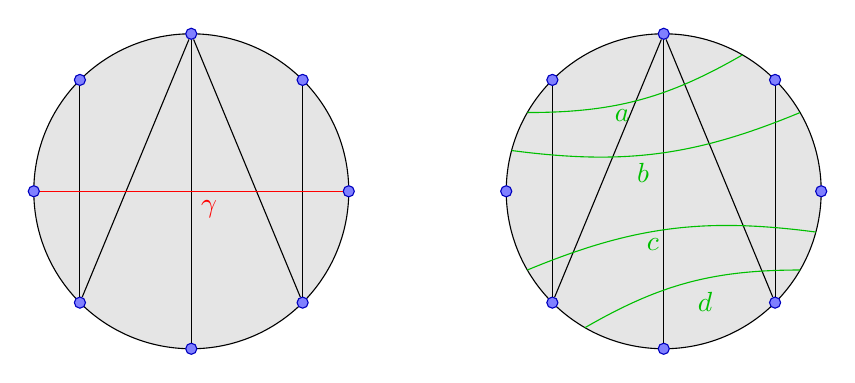
\begin{tikzpicture}[scale=1]
\begin{scope}[xshift=0cm]
	\draw[fill=black!10] (0,0) circle (2);
	\node[marked] (1) at (90:2) {};
	\node[marked] (2) at (45:2) {};
	\node[marked] (3) at (0:2) {};
	\node[marked] (4) at (-45:2) {};
	\node[marked] (5) at (-90:2) {};
	\node[marked] (6) at (-135:2) {};
	\node[marked] (7) at (-180:2) {};
	\node[marked] (8) at (135:2) {};
	\draw (8) to node[below] {} (6);
	\draw (6) to node[below] {} (1);
	\draw (1) to node[below] {} (5);
	\draw (1) to node[below] {} (4);
	\draw (4) to node[below] {} (2);
	\draw[red] (7) to node[below right] {$\gamma$} (3);
\end{scope}
\begin{scope}[xshift=6cm]
	\draw[fill=black!10] (0,0) circle (2);
	\node[marked] (1) at (90:2) {};
	\node[marked] (2) at (45:2) {};
	\node[marked] (3) at (0:2) {};
	\node[marked] (4) at (-45:2) {};
	\node[marked] (5) at (-90:2) {};
	\node[marked] (6) at (-135:2) {};
	\node[marked] (7) at (-180:2) {};
	\node[marked] (8) at (135:2) {};
	\draw (8) to node[below] {} (6);
	\draw (6) to node[below] {} (1);
	\draw (1) to node[below] {} (5);
	\draw (1) to node[below] {} (4);
	\draw (4) to node[below] {} (2);
	\draw[lamination,relative,out=-15,in=195] (150:2) to node[below left] {$a$} (60:2);
	\draw[lamination,relative,out=-15,in=195] (165:2) to node[below left] {$b$} (30:2);
%	\draw[lamination,relative] (195:2) to node[below right] {$c$} (15:2);
	\draw[lamination,relative,out=15,in=165] (210:2) to node[below left] {$c$} (-15:2);
	\draw[lamination,relative,out=15,in=165] (240:2) to node[below right] {$d$} (-30:2);
\end{scope}
%\begin{scope}[xshift=12cm]
%	\draw[fill=black!10] (0,0) circle (2);
%	\node[marked] (1) at (90:2) {};
%	\node[marked] (2) at (45:2) {};
%	\node[marked] (3) at (0:2) {};
%	\node[marked] (4) at (-45:2) {};
%	\node[marked] (5) at (-90:2) {};
%	\node[marked] (6) at (-135:2) {};
%	\node[marked] (7) at (-180:2) {};
%	\node[marked] (8) at (135:2) {};
%	\draw (8) to node[above] {$\scriptstyle -b$} (6);
%	\draw (6) to node[below] {$\scriptstyle b+c+d$} (1);
%	\draw (1) to node[above] {$\scriptstyle -d$} (5);
%	\draw (1) to node[below] {$\scriptstyle -a-b-c$} (4);
%	\draw (4) to node[above] {$\scriptstyle a+b$} (2);
%\end{scope}
%\begin{scope}[xshift=18cm]
%	\draw[fill=black!10] (0,0) circle (2);
%	\node[marked] (1) at (90:2) {};
%	\node[marked] (2) at (45:2) {};
%	\node[marked] (3) at (0:2) {};
%	\node[marked] (4) at (-45:2) {};
%	\node[marked] (5) at (-90:2) {};
%	\node[marked] (6) at (-135:2) {};
%	\node[marked] (7) at (-180:2) {};
%	\node[marked] (8) at (135:2) {};
%	\draw (8) to node[above] {$\scriptstyle -b-x$} (6);
%	\draw (6) to node[below left] {$\scriptstyle b+c+d+x+y$} (1);
%	\draw (1) to node[above] {$\scriptstyle -d$} (5);
%	\draw (1) to node[below right] {$\scriptstyle -a-b-c-x-y$} (4);
%	\draw (4) to node[above] {$\scriptstyle a+b+y$} (2);
%\end{scope}
\end{tikzpicture}
\end{center}
Read left to right, the non-boundary shear coordinates are as follows.
\[ S_1 = -a-b,\;\;\; S_2 = a+b+c,\;\;\; S_3 = d,\;\;\; S_4 = -b-c-d,\;\;\; S_5 = b\]
The admissible $a$ are $\{1,2,5\}$ and the admissible $b$ are $\{2,4,5\}$.
\[\begin{array}{|c|ccc|}
\hline 
\sum & 2 & 3 & 5 \\
\hline
1 & c  & c+d & 0 \\
2 & a+b+c & a+b+c+d & a+b \\
5 & 0 & 0 & b \\
\hline
\end{array} \]
The lemma asserts that the above sums are non-negative, and $\sum_1^5$ must be $0$.
\end{ex}

Consequently, the wall in $\mathbb{R}^\Delta$ associated to the I-beam defined by $\gamma$ is
\[ W_\gamma:= \left\{ v\in \mathbb{R}^\Delta : \sum_{i=1}^n S_i =0 \text{ and }\forall \text{ admissible }[a,b], \sum_{i=a}^b S_i \geq 0\right\} \]

\begin{rem}
These inequalities were reverse engineered from Bridgeland's work.
The marked arc $\gamma$ determines an $A_n$-quiver (the mutable quiver of the universal cover of the local neighborhood of $\gamma$), and this quiver has a unique irrep whose dimension vector is all $1$s. The admissible intervals are precisely the proper subreps of this representation, and the inequality is the stability condition.
\end{rem}

%\begin{proof}[Proof of Lemma \ref{lemma: inequalities}]
%We prove the lemma by induction on $n$ (the number of intersections between $\gamma$ and $\Delta$). Since $\gamma$ is not in $\Delta$, the base case is $n=1$. If $n=1$, then the first half of the lemma is trivial and the second half is the definition of the shear coordinate.
%
%Now, assume $\gamma$ and $\Delta$ intersect $n>1$ times, and assume the inductive hypothesis. Let $\gamma_1$ and $\gamma_2$ be the marked arcs such that
%\end{proof}

\newpage

\begin{thebibliography}{27}
\bibitem{GHKK}
M. Gross, P. Hacking, S. Keel, and M. Kontsevich,
\textit{Canonical bases for cluster algebras.}
Preprint, 2014. \texttt{arXiv:1411.1394}



\end{thebibliography}



\end{document}  